\documentclass[a4paper,11pt]{jsreport}
\usepackage[dvipdfmx]{graphicx,color,hyperref}
\PassOptionsToPackage{hyphens}{url}
\usepackage{pxjahyper}

% 数式
\usepackage{amsmath,amsfonts}
\usepackage{bm}
\usepackage{listings,plistings}
\usepackage{url}
\usepackage{courier}
\usepackage[top=20truemm,bottom=20truemm,left=25truemm,right=25truemm]{geometry}
\lstset{
   basicstyle={\ttfamily\small},
   frame=tRBl,
   framesep=10pt,
   breaklines=true,
   linewidth=17.5cm,
    lineskip=-0.5ex,
    tabsize=2,
	basewidth={0.65em,0.65em},
	language=Python,
}
% 画像
\usepackage[dvipdfmx]{graphicx}
\usepackage{here}
\usepackage{pdfpages} 
\usepackage{physics}

\usepackage{multicol}
\usepackage{moreverb}


\setlength{\columnsep}{4.5cm}

\begin{document}

\title{データベースシステムI\\最終レポート課題}
\author{筑波大学 情報学群 情報メディア創成学類 3年\\ 2022***** 田村 匠}
\date{\today}
\maketitle

\tableofcontents

\chapter{目的}
\section{はじめに}
今回の最終レポート課題では,私は「親父ギャクコロシアム」という
親父ギャグの投稿・評価が行えるWebアプリを作成した.

私は親父ギャクが大好きで,日常生活の中で思い付き,
発言してしまうことも多い.
その場合,多くは「寒い」「つまらない」といった評価をいただくことになる.
しかしながら,まれに「面白い」という評価をいただくこともある.

同じ親父ギャクにもかかわらず,面白さと寒さにギャグが分類されるのはなぜだろうか.
どのようにすれば,面白い親父ギャクのエッセンスを得ることができるだろうか.

そこで,私は親父ギャクを投稿し,「面白い」「寒い」の両軸で評価できる
「親父ギャクコロシアム」というWebサービスを開発することを思いついた.

親父ギャクを集積し,ユーザーが評価を行うことで,面白い,あるいは寒いギャグのデータがたまり,
将来的には,その傾向を分析することができるようになるだろう.

また,
実際にある程度実用に耐えうるユーザー認証・セッション管理
システムの構築や,NoSQLを用いたWebアプリの開発を経験してみたい
という技術的なモチベーションもこのトピックを選んだ理由の一つである.

\section{関連事例}
「親父ギャクコロシアム」のコンセプトと類似する既存Webサービスとしては,
ダジャレ・ステーション\cite{dajare-sta}が挙げられる.

ダジャレ・ステーションはダジャレを投稿し,評価・検索できるサービスである.
しかしながら,ダジャレ・ステーションと「親父ギャクコロシアム」には以下の違いがある.

\begin{itemize}
  \item 「ダジャレ」ではなく「親父ギャク」である.
  \item ダジャレ・ステーションは面白さのみを評価するが,親父ギャクには「面白い」と「寒い」の2つの評価軸が必要である.
\end{itemize}

また,何かを投稿し,評価するという概念は,一般的なSNSの概念と一致している.
一般的にこのようなサイトは,アカウント作成を経て,投稿・評価を行う.
また,このようなサイトは機能の追加削除が柔軟に行われる傾向がある.
そのため,データベース設計においては,機能の追加削除を容易に行える設計も
重要になるだろう.

今回の課題においては,このような先行事例を踏まえつつ,
データベースの設計・活用を主眼に置きながら,Webアプリの開発を行った.

\section{実装方法と制約事項}
サービスは,講義資料で示された通りに筑波大学のイントラネット内に構築した.
PythonとFlaskを用い,開発を行った.
データベースシステムとしてはMySQLとmongoDBを利用し,これらは
講義で用意されたホストを用いた.

開発にあたっては,実際にWebアプリを公開することが目的ではなく,
RDBMSあるいは,NoSQLデータベースシステムに関する理解を深めることが
目的であることを考慮し,機能・デザイン面においては最低限の実装のみを行った.

また,セキュリティの面においては,データベースシステムと密接にかかわる
SQLインジェクションなどに関しては重点的に対策を行ったが,
CSRF攻撃やログイン機能に対するブルートフォース攻撃などへの対策は完璧ではない状態となっている.

システムの起動は以下のコマンドで行う.
\begin{lstlisting}
$ python app.py
\end{lstlisting}
サイトは,\url{http://localhost:11067/}にホストされる.
is\_safe\_urlなど,動作にはpipにより追加のパッケージをインストールする必要がある.

\chapter{説明}
\section{機能説明・スクリーンショット}
親父ギャクコロシアムの機能は主に,以下の3つで説明される.
\begin{enumerate}
  \item ユーザー認証(セッション管理)
  \item 親父ギャグの投稿
  \item 親父ギャグの閲覧・評価
\end{enumerate}
この節では各機能について,スクリーンショットを提示しながら機能を説明する.

サイトは,\url{http://localhost:11067/}にホストされ,
トップページは図\ref{fig:top_unauth}のようになっている.

\begin{figure}[tb]
  \centering
  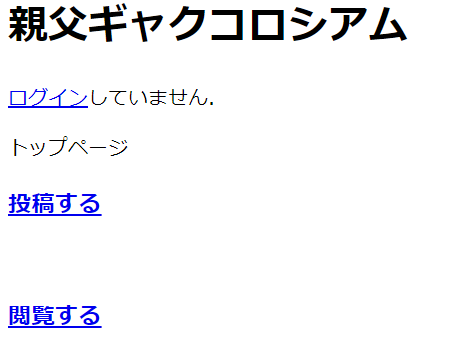
\includegraphics[width=8cm]{img/top_unauth.png}
  \caption{未ログイン状態のトップページ\label{fig:top_unauth}}
\end{figure}

\subsection{ユーザー認証}
閲覧機能以外はログインをしなければ,利用することができない.
未ログインの状態で,図\ref{fig:top_unauth}の「投稿する」などを押した場合,
警告メッセージとともに,図\ref{fig:login_post}のようなログイン画面に遷移する.
\begin{figure}[tb]
  \centering
  \includegraphics*[width=13cm]{img/login_post.png}
  \caption{ログインを促すメッセージ付きのログイン画面 \label{fig:login_post}}
\end{figure}

今回はアカウントを作成していないため,「ここから登録できます.」を
クリックして,アカウントを作成する.
図\ref{fig:register}のように,登録画面でアカウントを作成する.
\begin{figure}[tb]
  \centering
  \includegraphics*[width=13cm]{img/register.png}
  \caption{アカウント登録画面\label{fig:register}}
\end{figure}

アカウント作成時には,
\begin{itemize}
  \item ユーザIDは半角英数字とアンダーバーのみ利用でる.
  \item パスワードは5文字以上50文字以内で設定する.
\end{itemize}
というルールがあり,ルールを満たしていない場合は,
その旨が警告されアカウント作成はできない.

アカウントを作成すると,
図\ref{fig:top_auth}のように,ログイン状態で,
トップページに戻る.
\begin{figure}[tb]
  \centering
  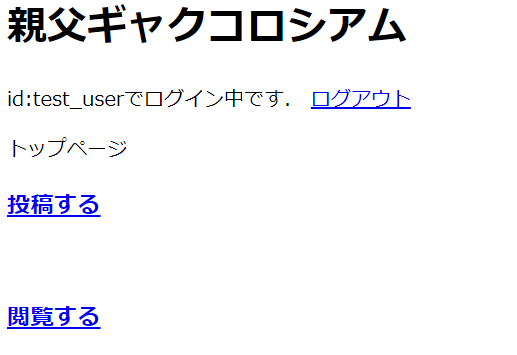
\includegraphics[width=8cm]{img/top_auth.png}
  \caption{ログイン状態のトップページ\label{fig:top_auth}}
\end{figure}

「ログアウト」を行い,「ログイン」から今設定した
ユーザID・パスワードでログインすることはもちろん可能である.

\subsection{親父ギャクの投稿}
ログイン状態の場合,投稿が可能である.
トップページの「投稿する」から図\ref{fig:post}の
投稿画面に遷移できる.
\begin{figure}[tb]
  \centering
  \includegraphics*[width=14cm]{img/post.png}
  \caption{投稿画面\label{fig:post}}
\end{figure}
「投稿」を押すと,図\ref{fig:post_confirm}の投稿確認画面へ遷移する.
ここで内容を確認し,前の画面に戻り修正することができる.
\begin{figure}[tb]
  \centering
  \includegraphics*[width=13cm]{img/post_confirm.png}
  \caption{投稿確認画面\label{fig:post_confirm}}
\end{figure}
問題がなければ,「投稿」を押す.すると,トップページに戻る.

\subsection{親父ギャグの閲覧・評価}
トップページから「閲覧する」をクリックすると,
図\ref{fig:view}のように,
投稿されたギャグを確認できる.
\begin{figure}[tb]
  \centering
  \includegraphics*[width=15cm]{img/view.png}
  \caption{閲覧・評価画面(寒い順でソートした場合)\label{fig:view}}
\end{figure}

ログイン状態であれば,面白い,あるいは,寒いの評価を
絵文字を押すことで行うことができる.
1度絵文字を押すと,絵文字は表示されなくなる.
1ユーザー1評価が原則となっている.

評価の数や投稿時間で,並び替えを行うことができる.

\section{使用したデータベースとデータベース設計}
このシステムでは,データベースシステムとして,
MySQLとmongoDBを利用をした.それぞれ,
MySQLはユーザー認証に,その他の機能にはmongoDBを利用した.
\subsection{ユーザー認証}
ユーザー認証はWebアプリのおいて最も基本的な機能の一つである.
ユーザー認証処理は高いセキュリティやACID特性が求められ,
一般的にはRDBMSで実装されることが多いように思える
\footnote{とはいえ,
負荷分散のためにNoSQLでユーザー認証/セッション管理をするという
事例もあるようだ.}.

そこで,MySQLを用いてユーザー認証(とセッション管理)の仕組みを構築することにした.

ここで,Webアプリにおいてはユーザー認証にはセッション管理セットになっている.
今回はflask-loginパッケージ\cite{flask-login}を用いてセッション管理を行った.
flask-loginでは,flaskのコード内で指定する
\begin{lstlisting}
  app.config["SECRET_KEY"]
\end{lstlisting}
を共通鍵として,ユーザーIDとタイムスタンプを暗号化し,
ユーザーのCookieに書き込むことで,ユーザーを識別するという
セッション管理を行っている.Cookieに書き込まれたタイムスタンプを利用し,一定時間経過すると,
セッションは無効となり,ログアウトされる.

セッション管理というと,ランダムに生成したセッションIDをDBで
管理するのが普通であるが,flask-loginはこれを上記の仕組みで簡略化し
DB無しで実装している.
この方法では,SECRET\_KEYが流出すると,
いくらでも不正にセッションが乗っ取られてしまうため,
SECRET\_KEYを確実に保護することが重要になる.

今回はflask-loginを利用するため,ユーザー認証でDBに保存する必要があるのは
ユーザーIDとそのパスワードのみである.

パスワードの保存にはセキュリティの向上のため,
ハッシュソルトを用いる.
パスワードをハッシュ化して保存すると,DBのデータが流出した場合に
パスワードが流出することを防ぐことができるが,
同じパスワードのハッシュ値は同じになるため,
統計的に使われやすいパスワードなどが推測されてしまう
(レインボー攻撃).
そこで.ユーザーごとにソルトといわれるランダムな情報を割り当てておき,
パスワードとソルトを合わせてハッシュ化するのが,
ハッシュソルトである.

MySQLに以下のようなテーブルを作成した.
\begin{lstlisting}
create table report_user (User_id varchar(128) NOT NULL PRIMARY KEY,Password char(224) NOT NULL, Salt char(32) NOT NULL); 
\end{lstlisting}
実際に,以下のようなデータが格納されている.
\begin{lstlisting}[language=C, basicstyle={\ttfamily\tiny}]
  mysql> select * from report_user ;
  +-----------+----------------------------------------------------------+----------------------------------+
  | User_id   | Password                                                 | Salt                             |
  +-----------+----------------------------------------------------------+----------------------------------+
  | hogepiyo  | 45153898f543d0f35709e4ad756492deb4642246c5003e10e37f2fba | 0826cff6199ee36a806401d645b0e891 |
  | takumi    | ce4cc9251a740ba81872e304fa587cd50c70e8bc00a706e469a800d2 | f217f794617dc8ba66239e40e5292a2f |
  | taro11    | 411e3dc221c36a08095b996b874f9ad8d4d7d5f89ad401162d699b0a | 9f8960992cf66cb2b3501d5b15c1bd58 |
  | test_user | e70eeceb396c425738368de510574d22b4197cf42b6320bc18ef9eb6 | cc734bff340a6e0ded0a488c5eca8030 |
  | User_1    | 31c143ba65e4cf800cb79fba07e311a715b6a78ff9a8402b424d4c39 | 074c83a17e1a5d3769da6400646ddb2b |
  | User_2    | 29794aa900222a5402321af5b033bdaa449823ad8391e619ea43d0a5 | 1219633b8e6fc413aeed11412f7297b0 |
  +-----------+----------------------------------------------------------+----------------------------------+
\end{lstlisting}
User\_1とUser\_2のパスワードはどちらも実際には
"qwerty"なのであるが,DBを見ただけでは推測できなくなっている.

ユーザー登録時には,暗号学的に安全な乱数発生器によって,
32文字のソルトが生成される.
設定されたパスワード,ソルトの順で文字列を結合し,
暗号学的ハッシュ関数であるSHA224を用いて,
結合文字列をハッシュ化する.
ユーザーID,ハッシュ化した文字列,ソルトをDBに挿入して登録が完了する.

ログイン時には,同じようにDBに保存されたソルトと入力されたパスワードを
ハッシュ化し.DBのハッシュ化文字列(Passwordカラム)と一致するかを検証する.

なお,
ユーザー入力されたユーザーIDやパスワードを
そのままクエリに利用すると,SQLインジェクションが発生する恐れがある.
しかし,ユーザーIDに使える文字種は厳しく制限されており,また,
パスワードはハッシュ化され安全な文字種のみとなるため,
SQLインジェクションが発生しない設計となっている.

\subsection{投稿並びに評価}
親父ギャクの投稿やその評価については,NoSQLである
mongoDBを用いた.

NoSQLを採用した理由としては,KVSのデータモデルが,RDBよりも,
評価機能等を実装する上で有利であると考えたからである.
評価数を記録するのみであればRDBMSでもシンプルに実装できるが,
どのユーザーがどの親父ギャクを評価したのかという記録は
関係データベースで表現した場合は中間テーブルなどを用いねばならず,
複雑になる.
対してKVSであれば,この構造は容易に表現できる.

また,
親父ギャクコロシアムのサービスは今後の機能拡張が期待されるサービスである.
現在は実装されていないが,投稿された親父ギャクに
コメントをつける機能が欲しくなるかもしれない.
コメントにいいね!を押したくなるかもしれない.
そのような機能拡張にRDBMSは不利である.

最終レポートで用いることができるNoSQLはmongoDBとRedisであるが,
後者はインメモリ型であり永続性の点から今回の用途には向かないため,
mongoDBを採用した.

\subsubsection{ドキュメントの設計}
1つの親父ギャグに関わるすべての情報は1つのドキュメントに格納されている.

mongoDBでは複数ドキュメントを対象とする操作はアトミックにならず,
単一ドキュメントを対象とする操作のみがアトミックとなる\cite{mongoAT}.
ゆえに,結果整合性を維持するためには,ある1つのドキュメントに
様々なデータを混載したほうが良いことになる.
\footnote{mongoDBのトランザクション機能を用いれば複数ドキュメントへの
操作をアトミックにできるが,その場合パフォーマンスは低下する.}

複数の親父ギャクを対象とする操作はほとんど想定されないため,
今回は親父ギャク1つにつき,1つのドキュメントとした.

では,実際のドキュメント構造を説明する.
\begin{lstlisting}
> db.gyagus.findOne();
{
        "_id" : ObjectId("62b6edd0e8286476dab6dfbc"),
        "gyagu" : "映像はええぞお・・・",
        "creater" : "takumi",
        "funs" : 3,
        "colds" : 4,
        "fun_users" : [
                "takumi",
                "User_1",
                "hogepiyo"
        ],
        "cold_users" : [
                "takumi",
                "User_1",
                "hogepiyo",
                "test_user"
        ],
        "created_at" : 1656155600.481688
}
\end{lstlisting}
親父ギャクは,ID,ギャグそのもの,UNIX時間で表されたUTCの投稿日時といった
基本的なデータを持っている.

ユーザーがどのギャグに評価をしたかという情報は,
ユーザーのドキュメントに持たせるという発想もできるが,その場合,
閲覧画面での評価数の取得が極めて面倒になってしまう.
そこで,今回は評価情報も親父ギャグドキュメントにすべて記載されている.

「面白い」の評価数と,評価したユーザーのリストである,funsとfun\_users,
同じく「寒い」の評価数と,評価したユーザーのリストである,coldsとcold\_users
が,評価情報を保存するデータである.
funs,coldsは,リストの長さを調べればその値が得られるので冗長なデータであるが,
リストの長さを調べる計算コストや,将来的な機能拡張を考慮し,
冗長な設計とした.例えば,プレミアム・ユーザーは一般ユーザーの
3倍評価可能であるといった機能を実装するかもしれない.先述したように,
単一ドキュメントに対する操作はすべてアトミックであるから,
正規化されていない冗長なデータがあっても
パフォーマンスや整合性には影響しない.

親父ギャグドキュメントはコレクションgyagusに格納され,データベースが構成される.

\chapter{自己評価}
\section{目的は達成されたか?}
\subsection{プロダクトの目的}
今回の目的は,親父ギャグを投稿し,それに対して「面白い」「寒い」の
評価を行うというWebアプリの作成であった.
最低限の機能は実装され,問題なく動作した.
その点で,目的はおおむね達成されたといえよう.

しかしながら,大量アクセス時,あるいは,大量にデータがある場合に,
正常に動作するかに関しては自信がない.
例えば,評価ボタンは評価済みの場合は表示されないが,
これはすべての親父ギャグドキュメントに対して,
評価済みリスト内に自身のユーザーIDが存在しないかをチェックしている.
これは計算コストのかかる手法であり,データ数や評価数が増えた場合,
閲覧ページの読み込みに途方もない時間がかかる可能性が高い.

\subsection{技術的なモチベーション}
また,技術的なモチベーションに関しても,
ログイン認証機能の実装や,NoSQLの活用など,
おおむね目標は達成されたは満たされたといえる.

一方で,flask-loginはセッション管理を伴わない極めて簡素な
ユーザー認証を提供しており,ログイン認証機能の実装の本質を
経験したとは言い難い.また,NoSQL,mongoDBの活用も
シンプルな範囲にとどまり,多くの機能を経験したとは言い難いだろう.
\\

プロダクトとしての目的や,技術上のモチベーションにおいて不十分な点は
今後の課題のひとつとして,取り組んでいくことになる.
\section{今後の課題}
今後の課題としては,上記で挙げられた目的に対する不十分な点のほかに,
第1章において「制約事項」とした,機能・デザイン・セキュリティの問題がある.
\subsection{機能}
機能面の課題としては,親父ギャグに対してコメントを投稿したり,その
コメントを評価する機能を検討している.
mongoDBを用いているため,機能拡張はある程度容易であるだろう.
\subsection{デザイン}
今後の課題として最も重大なものは,Webデザインである.現在のデザインは
本当にひどいものであり,実用に供しない.実際のサービスとして展開するのは,
立派なデザインが必要になるだろう.
\subsection{セキュリティ}
flask-loginのセッション管理手法は脆弱であり,より高度な手法を採用すべきである.
また,ある程度の対策は施したが,XSS攻撃やCSRF攻撃におそらくアプリは脆弱である.

公開されているユーザーidとパスワードでログインするという設計もセキュリティ的には
危険であり,また,複数回ログインに失敗した場合のロック機能などもない.
これらセキュリティの問題は永遠の課題となるだろう.

\renewcommand{\bibname}{参考文献}
\bibliographystyle{jplain}
\bibliography{bibtex}

\end{document}